\section{Einleitung}

\begin{frame}[c]
	\frametitle{Einleitung}

??

\end{frame}

\begin{frame}[c]
	\frametitle{Brute-Force-Angriff}

	Grafik mit Verschlüsselung, Entschlüsselung, Brute-Force-Angriff 

	//Durch Eigenschaften der Nachricht lässt sich ein Treffer erkennen (natürlichsprachlich, Primzahl, festes Dokumentenformat)

\end{frame}

\begin{frame}[c]
	\frametitle{Verwendete Passwörter}

	\begin{center}
		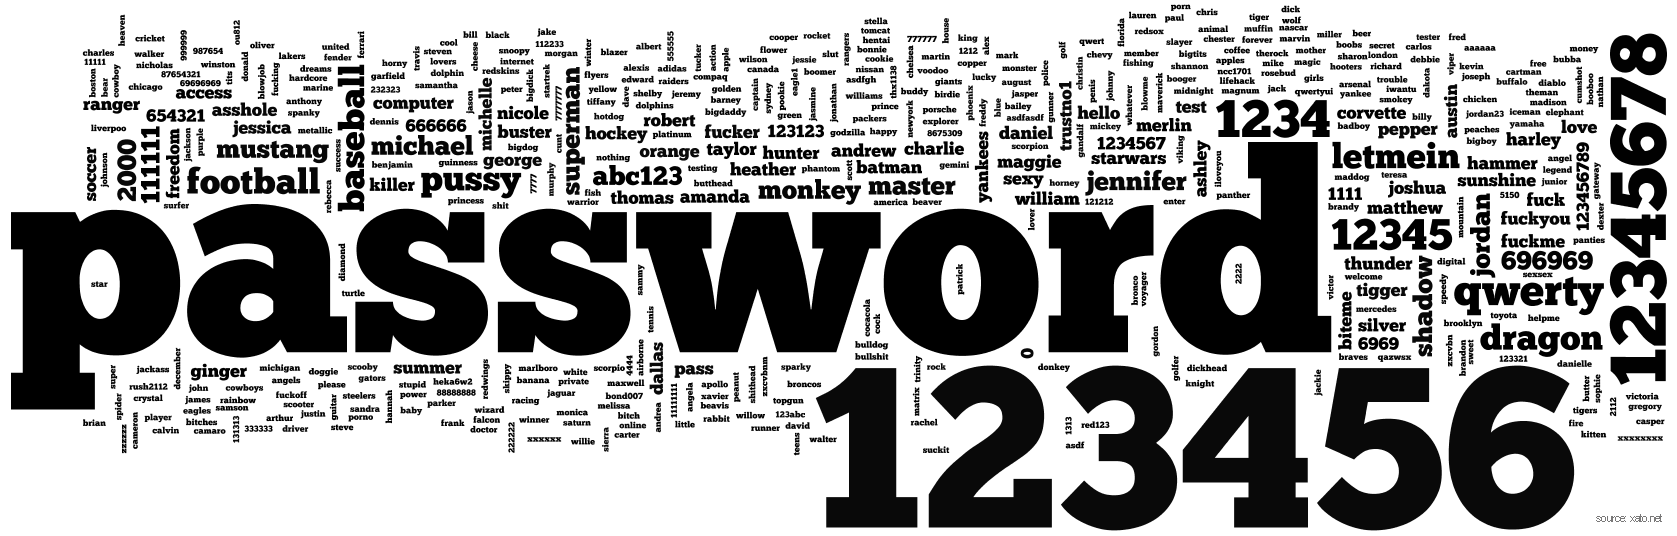
\includegraphics[width=\textwidth]{pic/passwordscloud.png}

		\emph{https://xato.net/wp-content/xup/passwordscloud.png}
	\end{center}
\end{frame}

\begin{frame}[c]
	\frametitle{Honey Encryption}

	\begin{center}
		"`Honey Encryption wurde entwickelt, um Ciphertexte zu generieren, die bei Entschlüsselung mit einem falschen Schlüssel zu einem plausibel wirkenden, aber unechten Klartext führen."'

		\vspace*{1cm}

		\textit{ [A. Juels, T. Ristenpart:\\ Honey Encryption - Security Beyond the Brute-Force Bound]}
	\end{center}
\end{frame}